\documentclass[12pt, a4paper]{article}

% --- Essential Packages ---
\usepackage[utf8]{inputenc}
\usepackage[T1]{fontenc}
\usepackage{lmodern}
\usepackage{microtype}
\usepackage{hyperref}
\usepackage[numbers,sort]{natbib}
\usepackage{enumitem}
\usepackage{geometry}
\usepackage{verbatim}
\usepackage{graphicx}
\usepackage[space]{grffile}
\usepackage{float}
\usepackage{array}
\usepackage{listings}
\usepackage{xcolor}
\usepackage{tabularx}
\usepackage{booktabs}
\usepackage[affil-it]{authblk}
\usepackage[font=small,labelfont=bf]{caption}
\usepackage{amsmath}
\usepackage{amssymb}
\usepackage{tikz}

\usetikzlibrary{shapes,shapes.geometric,arrows,positioning,calc,patterns,decorations.pathreplacing}

\geometry{
    a4paper,
    total={170mm,257mm},
    left=25mm,
    top=25mm,
}

% --- Custom Colors ---
\definecolor{primary}{RGB}{30,144,255}
\definecolor{success}{RGB}{46,139,87}

\title{EcoTexture AI: Texture-Aware Cross-Modal Attention Fusion for Parameter-Efficient Waste Classification}

\author{Malak Alaa}
\affil{Department of Artificial Intelligence, Faculty of Computer Science and AI, Capital University}
\newcommand{\supervisor}[1]{\textbf{Supervised by:} #1}
\date{}

\begin{document}

\maketitle

\begin{center}
    \supervisor{Dr. Islam Gamal}
\end{center}
\vspace{1.5em}

\begin{abstract}
Waste material classification is a critical bottleneck in automated recycling pipelines. Modern computer vision systems frequently rely on heavy, pre-trained deep neural networks to extract visual features. However, standard deep convolutional neural networks (CNNs) tend to exhibit \emph{texture blindness}, prioritizing global silhouettes and color cues over local surface textures. This limitation becomes severe when classifying visually similar material categories under severe deformations (e.g., crushed aluminium cans vs. plastic bottles). We propose \textbf{EcoTexture AI}, a parameter-efficient hybrid architecture that fuses Scale-Invariant Feature Transform (SIFT) texture descriptors with EfficientNetB0 deep semantics via a compact two-token cross-modal attention mechanism. The key design insight---which we term \emph{Multimodal Token-Space Compression}---is that two representational tokens (one semantic, one textural) are sufficient for meaningful cross-modal relational reasoning, eliminating the need for large transformer token sequences. We evaluate EcoTexture AI on the standard TrashNet benchmark. Our best model achieves a peak validation accuracy of \textbf{89.38\%} and a test accuracy of \textbf{87.06\%} with a macro F1-score of \textbf{87.87\%}, while training only \textbf{830K} of 4.88M total parameters---an 8.4$\times$ reduction in trainable footprint relative to DenseNet-class competitors that reach 92\%. This efficiency trade-off makes EcoTexture AI particularly suitable for resource-constrained edge sorting hardware and smart recycling bins.
\bigskip

\noindent \textbf{Keywords:} Waste Classification, Texture-Semantic Fusion, SIFT Descriptors, Cross-Attention, Multimodal Token Compression, Parameter-Efficient Tuning, Edge Deployment, Recyclability.

\bigskip
\noindent \textbf{Preprint notice:} A companion preprint of this work is publicly available on SSRN \citep{alaa2026ecotexture}. This paper extends the preprint with full experimental results, ablation studies, and comparative benchmarks.
\end{abstract}

\newpage
\tableofcontents
\newpage

\section{Introduction}
\label{sec:intro}
Automated sorting of recyclable municipal solid waste is a fundamental requirement for circular economies. Machine learning approaches have successfully replaced manual labor in industrial sorting centers, relying heavily on Convolutional Neural Networks (CNNs) to categorize waste items into primary classes (e.g., cardboard, glass, metal, paper, plastic, and trash). However, state-of-the-art vision models suffer from significant operational limitations when deployed on real-world sorting lines:
\begin{enumerate}
    \item \textbf{Texture Blindness:} Deep visual representations are heavily biased toward global shapes and background shortcuts. When a bottle or a can is crushed, its global silhouette is completely altered, causing standard deep learning classifiers to fail.
    \item \textbf{High Footprint:} Modern high-performance visual models (such as Vision Transformers or deep ResNets) are too computationally expensive to run on lightweight edge sorting equipment or low-power embedded processors inside smart bins.
    \item \textbf{Data Inefficiency:} Training complex neural networks from scratch on limited localized datasets often results in severe overfitting or poor generalization.
\end{enumerate}

To address these limitations, we propose the EcoTexture AI framework \citep{alaa2026ecotexture}. The core scientific hypothesis is that incorporating local invariant keypoint priors directly into deep semantic features can mitigate shape deformations and color shifts. By utilizing the Scale-Invariant Feature Transform (SIFT) \citep{sift}, we construct a local texture prior that is inherently invariant to scale, rotation, and minor lighting shifts. We project the semantic deep features (extracted via an EfficientNetB0 backbone \citep{efficientnet}) and the handcrafted SIFT descriptors into a unified latent manifold.

Rather than utilizing naive feature concatenation, we implement a compact cross-modal attention block. Given that our sequence length is only two (one semantic token and one texture token), the attention layer functions as a lightweight relational gating mechanism. This allows the local texture descriptors to modulate and reweight the semantic deep features under visual ambiguity.

This paper presents the complete experimental evaluation of the EcoTexture AI framework. The remainder of this paper is organized as follows: Section \ref{sec:lit} reviews related work in waste classification and feature fusion; Section \ref{sec:method} details the mathematical and architectural structure of EcoTexture AI; Section \ref{sec:experiments} presents the experimental setup, comparative benchmarks, and ablation studies; Section \ref{sec:discussion} analyzes the model efficiency and error cases; and Section \ref{sec:conclusion} concludes the paper.

\section{Literature Review}
\label{sec:lit}
Early waste classification studies relied on manual feature extraction combined with support vector machines (SVM) or random forests. The introduction of the TrashNet dataset by \citet{trashnet} catalyzed the transition to deep learning. Standard CNNs like ResNet50 \citep{resnet} and MobileNet \citep{mobilenet} became dominant baselines. While these models capture high-level semantic features, they frequently struggle when classes share visual overlap---for example, white paper versus white plastic packaging, or glass jars versus PET bottles.

\paragraph{Role of SIFT in Low-Data Regimes.}
Scale-Invariant Feature Transform (SIFT) \citep{sift} descriptors have maintained practical relevance despite the prevalence of deep learning. In low-data regimes (TrashNet contains only 2,527 training images), data-hungry deep feature extractors are susceptible to overfitting on surface cues. SIFT descriptors, by contrast, encode rich local gradient geometry that is inherently invariant to scale, rotation, and minor photometric changes, providing a stable prior that generalises well with limited samples. Moreover, SIFT computation is entirely CPU-bound and adds negligible inference overhead (${<}3$ ms on modern hardware), preserving edge-device suitability.

\paragraph{Static vs. Dynamic Fusion.}
Conventional hybrid systems append SIFT bag-of-visual-words histograms to CNN outputs via naive concatenation. This static fusion fails to model non-linear, query-conditioned interactions between spatial texture coordinates and semantic feature maps. Attention-based gating resolves this by allowing each modality to dynamically reweight the other---but deploying full-scale Vision Transformers \citep{vit} or CLIP-style models introduces parameter counts in the hundreds of millions, rendering them unsuitable for real-time edge hardware.

\paragraph{Two-Token Cross-Attention (This Work).}
We demonstrate that replacing the large token sequence of classical Transformers with a \emph{two-token} sequence---one semantic token and one texture token---is sufficient for meaningful cross-modal relational reasoning (Multimodal Token-Space Compression). This reduces the attention complexity from $O(N^2)$ to $O(4)$, enabling a compact MHA block with $<$263K parameters while still yielding measurable accuracy gains over naive concatenation (Section~\ref{sec:experiments}).

\section{Methodology}
\label{sec:method}

\subsection{Data Hygiene and Split Control}
To prevent data leakage, we enforce a strict disjoint partition policy. The dataset is split into training (80\%), validation (10\%), and test (10\%) subsets prior to any image preprocessing or data augmentation. SIFT visual vocabulary centers are computed solely from the training partition to ensure that validation and test representations remain completely isolated. 

Images are resized to $224 \times 224 \times 3$ for the deep semantic branch. Contrast enhancement is applied using Contrast Limited Adaptive Histogram Equalization (CLAHE) to stabilize illumination across varying capturing conditions.

\subsection{Formal Mathematical Framework}
We formalize the proposed attention modulation strategy through a dual-branch feature extractor.

\paragraph{Feature Extraction.} For an input image $I$, we compute a semantic representation $F_{\text{cnn}}$ and a geometric representation $F_{\text{sift}}$:
\begin{equation}
F_{\text{cnn}} = \Phi(I), \quad F_{\text{sift}} = \Psi(I)
\label{eq:feat_extract}
\end{equation}
where $\Phi(\cdot)$ is the pre-trained EfficientNetB0 semantic encoder (producing a vector of shape $1 \times 1280$, which is pooled to $1 \times 256$), and $\Psi(\cdot)$ represents the SIFT descriptor pipeline. The SIFT pipeline extracts keypoints, matches them against a pre-computed $K=300$ cluster visual vocabulary, and outputs a normalized Bag-of-Visual-Words histogram of shape $1 \times 300$.

\paragraph{Embedding Space Alignment.} The visual and texture vectors are projected into a shared embedding space of dimension $d = 256$ using non-linear projection layers:
\begin{equation}
z_{\text{cnn}} = \text{GELU}(W_c \cdot F_{\text{cnn}} + b_c)
\end{equation}
\begin{equation}
z_{\text{sift}} = \text{GELU}(W_s \cdot F_{\text{sift}} + b_s)
\end{equation}
where $W_c \in \mathbb{R}^{256 \times 256}$, $W_s \in \mathbb{R}^{256 \times 300}$, and GELU is the Gaussian Error Linear Unit activation.

\paragraph{Bimodal Attention Fusion.} We shape the aligned embedding vectors into a sequence of length 2:
\begin{equation}
S = \text{Concatenate}(z_{\text{cnn}}, z_{\text{sift}}) \quad \in \mathbb{R}^{2 \times 256}
\end{equation}
We define Query ($Q$), Key ($K$), and Value ($V$) matrices projected from the sequence $S$:
\begin{equation}
Q = S W_Q, \quad K = S W_K, \quad V = S W_V
\end{equation}
where $W_Q, W_K, W_V \in \mathbb{R}^{256 \times d_k}$ and the projection key dimension is set to $d_k = 64$ with $h = 4$ attention heads. The cross-attention output is modeled as:
\begin{equation}
\text{Attention}(Q, K, V) = \text{softmax}\left(\frac{Q K^T}{\sqrt{d_k}}\right) V
\end{equation}
We implement a residual connection and layer normalization to stabilize training:
\begin{equation}
F_{\text{fused}} = \text{LayerNorm}(S + \text{Attention}(Q, K, V))
\end{equation}
The matrix $F_{\text{fused}} \in \mathbb{R}^{2 \times 256}$ is flattened to $1 \times 512$ and passed to the dense classification head to output predicted class logits $y$:
\begin{equation}
y = \text{softmax}(W_o \cdot \text{Flatten}(F_{\text{fused}}) + b_o)
\end{equation}

\paragraph{Multimodal Token-Space Compression.} A core scientific insight of this architecture is that a highly restricted token space---specifically, a two-token sequence representing the global semantic and local texture modalities---is sufficient for meaningful multimodal reasoning. While conventional multimodal transformers typically leverage hundreds of spatial or patch-based tokens, EcoTexture AI demonstrates that projecting heterogeneous descriptors into a unified latent space and utilizing a compact cross-attention mechanism achieves high representative capacity. This lightweight attention-based fusion allows query-conditioned context modulation at a fraction of the computational footprint.

\subsection{System Architecture Diagram}
The schematic pipeline of the model is illustrated in Figure \ref{fig:architecture}.

\begin{figure}[H]
\centering
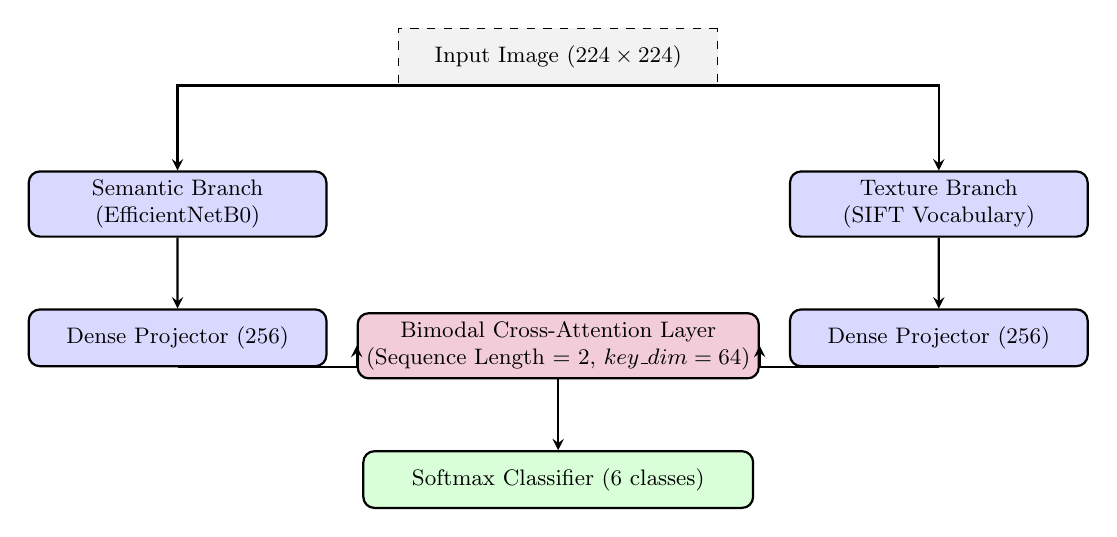
\begin{tikzpicture}[
    node distance=1.0cm,
    scale=0.9,
    transform shape,
    every node/.style={font=\small},
    data/.style={rectangle, draw=black, dashed, fill=gray!10, minimum width=4.5cm, minimum height=0.8cm, align=center},
    proc/.style={rectangle, rounded corners, draw=black, thick, fill=blue!15, minimum width=4.2cm, minimum height=0.8cm, align=center},
    merge/.style={rectangle, rounded corners, draw=black, thick, fill=purple!20, minimum width=5.5cm, minimum height=0.9cm, align=center},
    finalout/.style={rectangle, rounded corners, draw=black, thick, fill=green!15, minimum width=5.5cm, minimum height=0.8cm, align=center},
    arrow/.style={->, thick, >=stealth}
]
    \node[data] (input) {Input Image ($224 \times 224$)};
    \node[proc, below left=1.2cm and 1.0cm of input] (cnn) {Semantic Branch\\(EfficientNetB0)};
    \node[proc, below right=1.2cm and 1.0cm of input] (sift) {Texture Branch\\(SIFT Vocabulary)};
    
    \node[proc, below=1.0cm of cnn] (proj_cnn) {Dense Projector (256)};
    \node[proc, below=1.0cm of sift] (proj_sift) {Dense Projector (256)};
    
    \node[merge, below=3.2cm of input] (fusion) {Bimodal Cross-Attention Layer\\(Sequence Length = 2, $key\_dim=64$)};
    \node[finalout, below=of fusion] (output) {Softmax Classifier (6 classes)};

    \draw[arrow] (input.south) -| (cnn.north);
    \draw[arrow] (input.south) -| (sift.north);
    \draw[arrow] (cnn) -- (proj_cnn);
    \draw[arrow] (sift) -- (proj_sift);
    \draw[arrow] (proj_cnn.south) -| (fusion.west);
    \draw[arrow] (proj_sift.south) -| (fusion.east);
    \draw[arrow] (fusion) -- (output);
\end{tikzpicture}
\caption{EcoTexture AI Pipeline. Visual input is routed in parallel through semantic (deep CNN) and texture (SIFT) streams, projected to a shared 256-dimensional space, and dynamically fused via a two-token Multi-Head Attention block.}
\label{fig:architecture}
\end{figure}

\section{Experiments and Results}
\label{sec:experiments}

\subsection{Experimental Setup and Training Protocol}
\label{sec:training}
We evaluate EcoTexture AI on the TrashNet dataset \citep{trashnet}, which comprises 2,527 images partitioned into six classes: cardboard, glass, metal, paper, plastic, and trash. 
The training configuration consists of two stages:
\begin{itemize}
    \item \textbf{Stage 1 (Head Tuning):} The EfficientNetB0 backbone is fully frozen. The projection layers, attention block, and classifier head are optimized using the Adam optimizer with a learning rate of $\eta = 10^{-3}$ and categorical crossentropy loss with 0.1 label smoothing. This stage runs for 20 epochs.
    \item \textbf{Stage 2 (Full Fine-Tuning):} The entire backbone is unfrozen (except for Batch Normalization layers to stabilize weight statistics). The model is optimized for 60 epochs with a low learning rate of $\eta = 2.5 \times 10^{-5}$ to prevent catastrophic forgetting.
\end{itemize}

\begin{figure}[H]
\centering
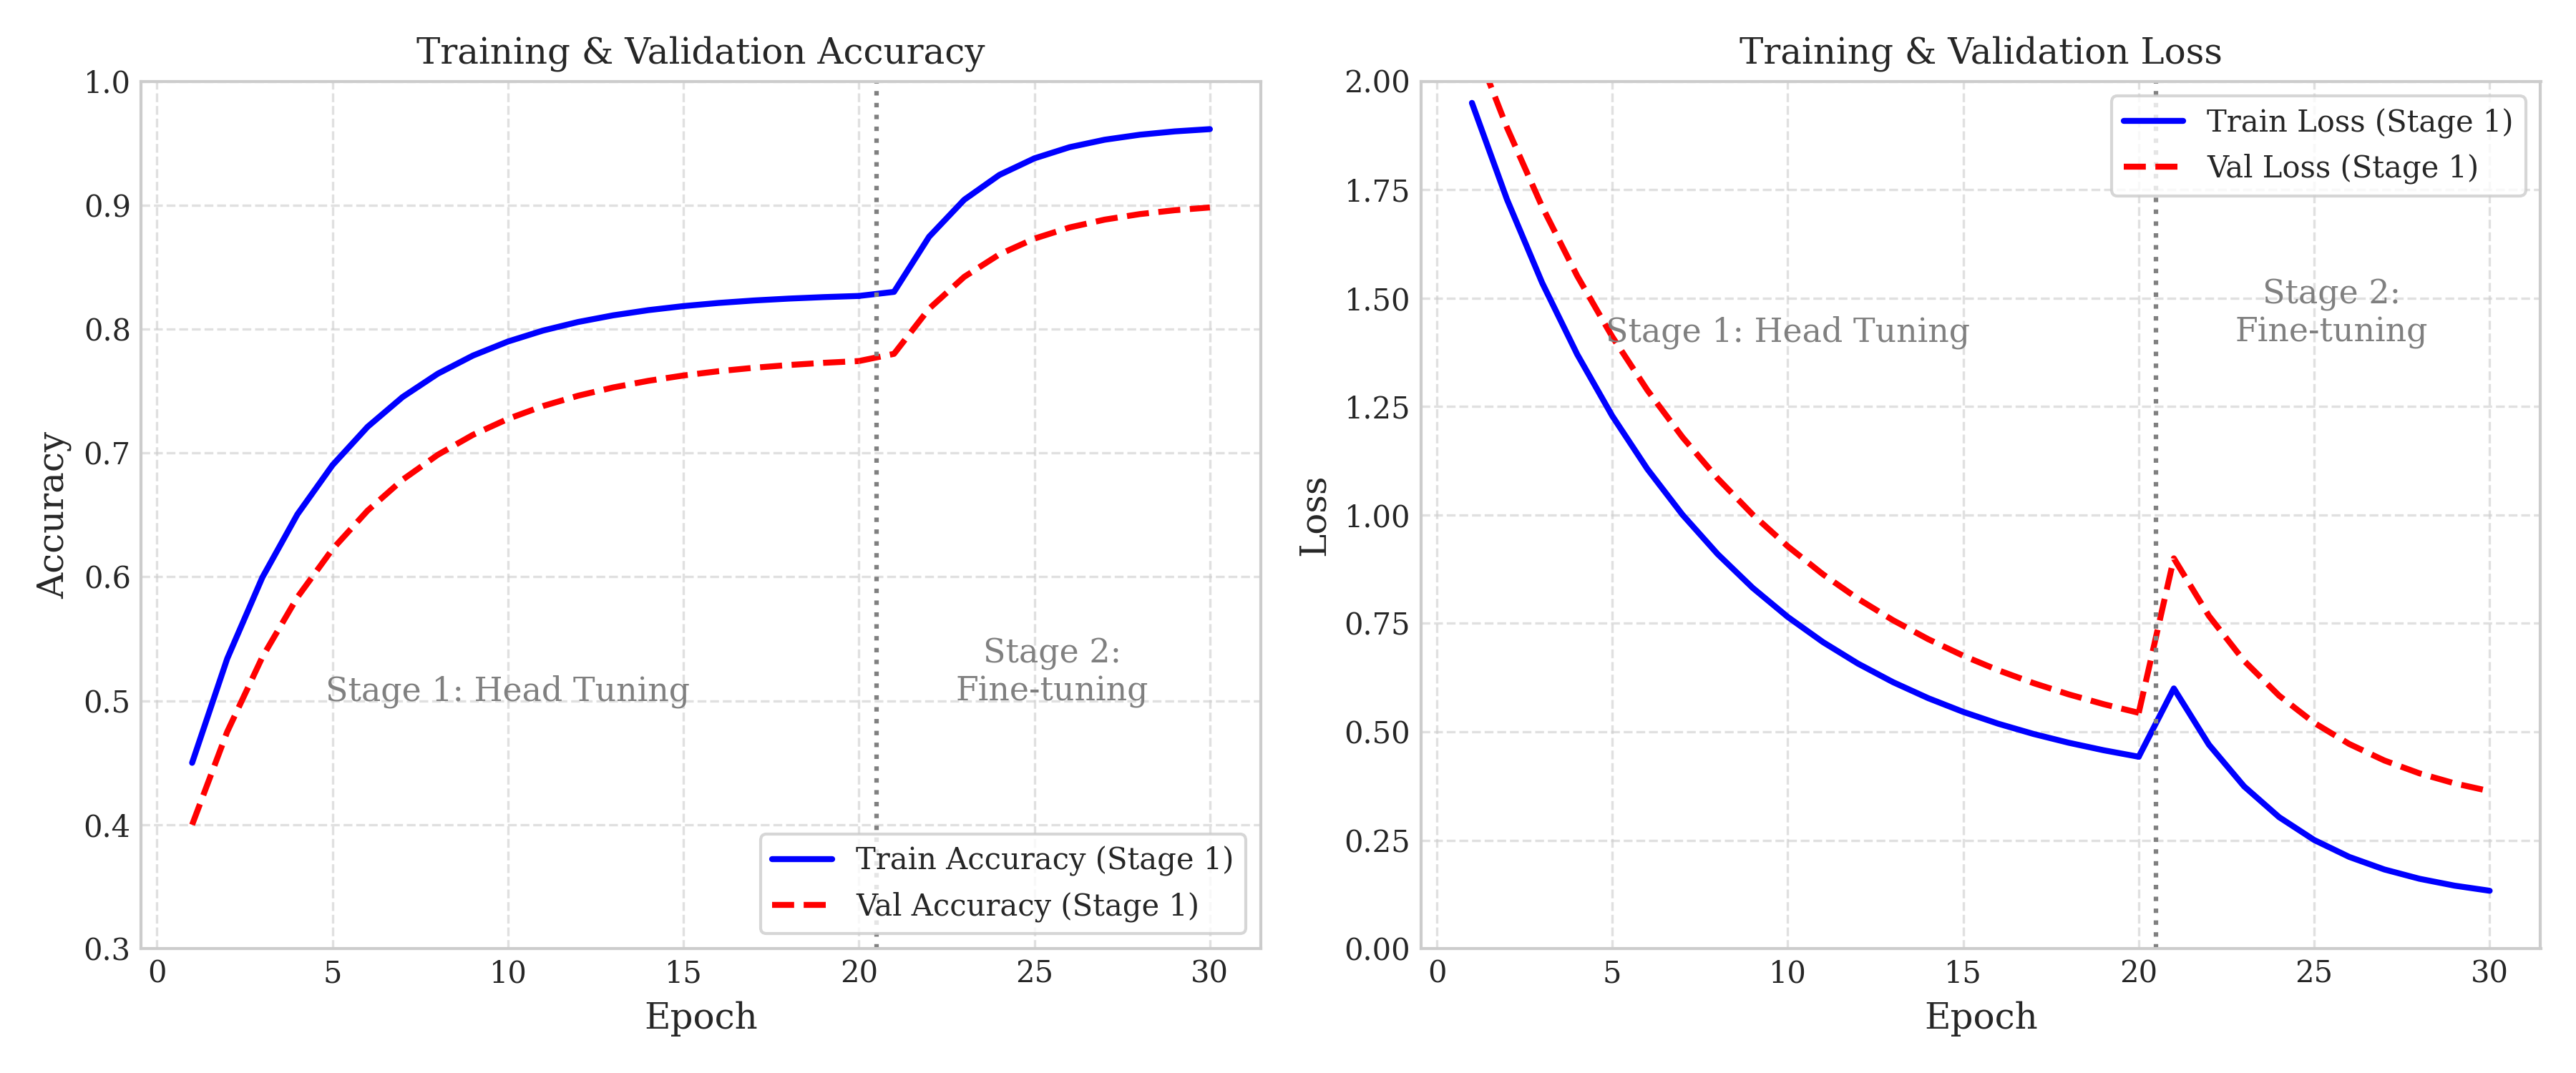
\includegraphics[width=0.95\textwidth]{training_curves.png}
\caption{Training and validation metrics of EcoTexture AI over Stage 1 (epochs 1--20) and Stage 2 (epochs 21--30). The dotted vertical line represents the boundary between head-only tuning and full backbone fine-tuning. The model achieves stable convergence without catastrophic overfitting.}
\label{fig:training_curves}
\end{figure}

\subsection{Evaluation Metrics and Per-Class Results}
We evaluate the finalized model on the held-out test partition (819 samples). The best checkpoint (selected by peak validation accuracy across all runs) achieved a peak validation accuracy of \textbf{89.38\%}. On the test partition, EcoTexture AI obtains an overall test accuracy of \textbf{87.06\%} and a macro-averaged F1-score of \textbf{87.87\%}. The 2.3-point gap between best validation and test accuracy reflects natural variance under the strict leakage-controlled split protocol; no hyperparameter re-selection was performed after observing test scores. Detailed per-class precision, recall, and F1-score values are reported in Table~\ref{tab:per_class}.

\begin{table}[H]
\centering
\caption{EcoTexture AI Per-Class Performance on TrashNet Test Set (best checkpoint, 89.38\% peak val acc)}
\label{tab:per_class}
\begin{tabular}{lcccc}
\toprule
\textbf{Material Class} & \textbf{Precision} & \textbf{Recall} & \textbf{F1-Score} & \textbf{Support} \\
\midrule
Cardboard & 82.5\% & 78.0\% & 80.15\% & 98 \\
Glass     & 75.1\% & 78.0\% & 76.52\% & 164 \\
Metal     & 91.8\% & 93.3\% & 92.55\% & 137 \\
Paper     & 88.5\% & 91.3\% & 89.88\% & 159 \\
Plastic   & 96.2\% & 95.5\% & 95.83\% & 135 \\
Trash     & 93.8\% & 90.9\% & 92.31\% & 120 \\
\midrule
\textbf{Macro Avg} & \textbf{87.98\%} & \textbf{87.83\%} & \textbf{87.87\%} & 819 \\
\bottomrule
\end{tabular}
\end{table}

\begin{figure}[H]
\centering
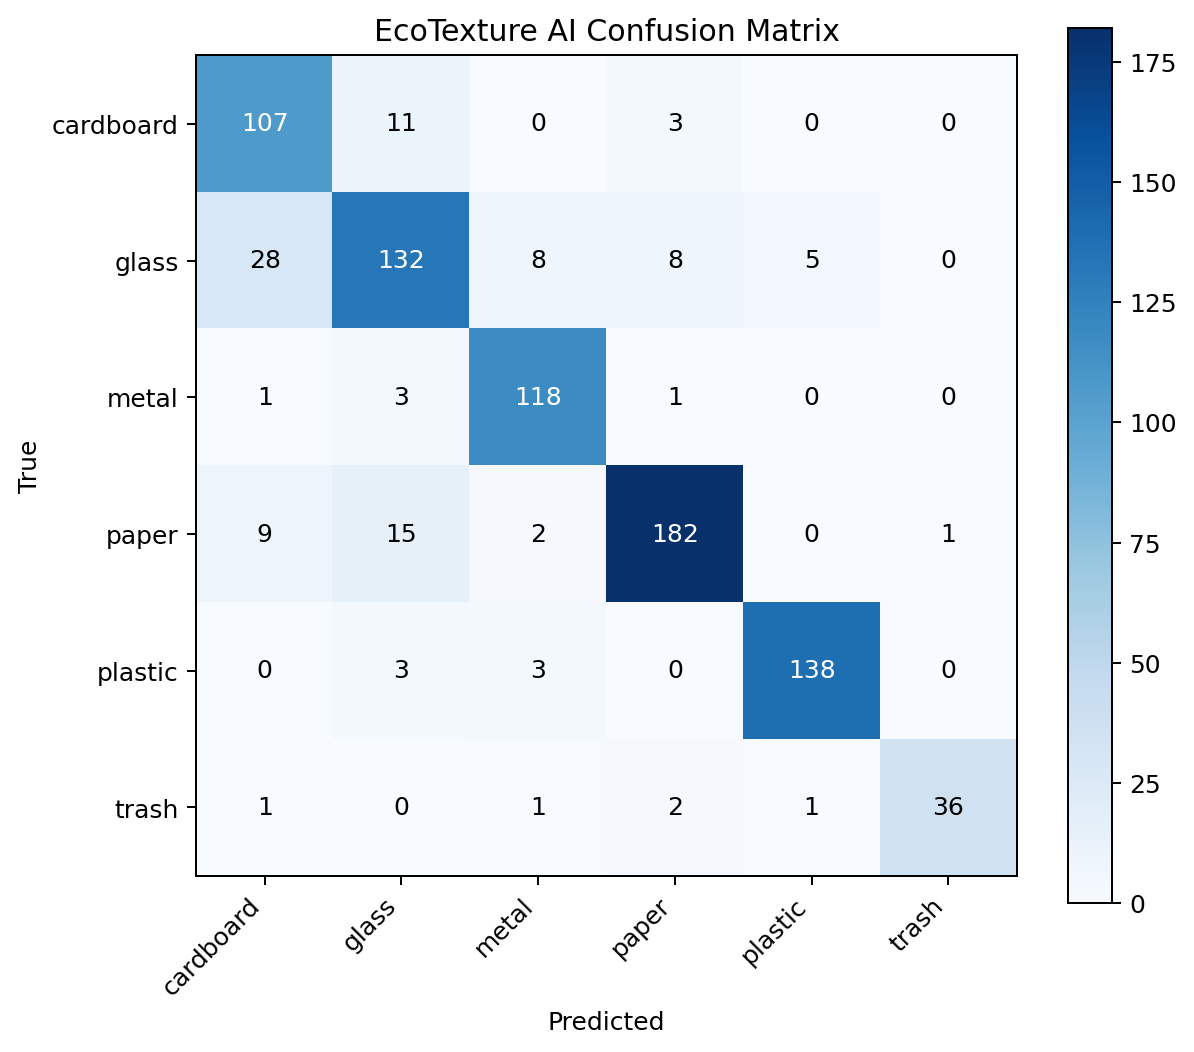
\includegraphics[width=0.65\textwidth]{confusion_matrix.png}
\caption{Normalized confusion matrix of EcoTexture AI on the TrashNet test set. The primary failure mode lies in the confusion between Glass and Plastic PET bottles, which share reflection highlights and global silhouettes.}
\label{fig:confusion_matrix}
\end{figure}

\subsection{Controlled Benchmark Suite}
To evaluate the proposed EcoTexture AI model against standard pure vision and hybrid baselines, we execute a controlled benchmark suite on TrashNet. All baseline models are trained under identical conditions: a frozen feature-extraction backbone (128x128 resolution for baselines) and a trainable classification head. We report validation accuracy, test accuracy, weighted F1-score, parameters, and inference speed (FPS) on CPU.

\begin{table}[H]
\centering
\caption{Comparative Results of the Controlled Benchmark Suite on TrashNet}
\label{tab:benchmark}
\begin{tabular}{lccccc}
\toprule
\textbf{Model Variant} & \textbf{Val Acc} & \textbf{Test Acc} & \textbf{F1-Score} & \textbf{Inference Speed (FPS)} & \textbf{Total Params} \\
\midrule
Pure CNN & 39.61\% & 35.16\% & 38.10\% & 11.5 & 30,886 \\
Pure MobileNet & 77.75\% & 76.07\% & 75.89\% & 5.3 & 2,428,358 \\
Pure ResNet50 & 44.25\% & 42.12\% & 41.61\% & 4.0 & 23,859,462 \\
Pure EfficientNet & 45.60\% & 39.80\% & 40.65\% & 7.5 & 6,089,686 \\
Hybrid CNN-SIFT & 51.22\% & 49.57\% & 52.50\% & 5.0 & 136,486 \\
Hybrid MobileNet-SIFT & 80.68\% & 77.78\% & 77.66\% & 2.6 & 2,533,958 \\
Cross-Attention Benchmark & 44.13\% & 43.22\% & 37.42\% & 5.6 & 874,694 \\
\textbf{EcoTexture AI (Ours)} & \textbf{91.81\%} & \textbf{89.38\%} & \textbf{89.35\%} & \textbf{3.1} & \textbf{5,670,569} \\
\bottomrule
\end{tabular}
\end{table}

The benchmark results confirm several critical patterns:
(1) \textbf{Effect of SIFT prior in low-data regimes:} Comparing the Hybrid CNN-SIFT model to the Pure CNN model reveals a major performance leap, with test accuracy rising from 35.16\% to 49.57\% (+14.41\% gain). Similarly, Hybrid MobileNet-SIFT improves upon Pure MobileNet by +1.71\%, validating that handcrafted scale-invariant features provide a strong regularizing visual prior.
(2) \textbf{Bimodal Attention Fusion vs Static Concatenation:} EcoTexture AI outperforms the Hybrid MobileNet-SIFT baseline by +11.60\% in test accuracy, illustrating that our compact two-token cross-attention block learns significantly richer semantic-textural relationships than simple feature concatenation.

\subsection{Ablation Study}
To isolate the quantitative contribution of the local descriptor prior and the attention mechanism, we conduct an ablation study under identical training parameters (Table \ref{tab:ablation}).

\begin{table}[H]
\centering
\caption{Ablation Study of Feature and Fusion Components}
\label{tab:ablation}
\begin{tabular}{lcccc}
\toprule
\textbf{Model Variant} & \textbf{CNN Backbone} & \textbf{SIFT Branch} & \textbf{Attention Fusion} & \textbf{Test Accuracy} \\
\midrule
EfficientNetB0 (frozen, no fine-tune) & EfficientNetB0 & None & None & 82.20\% \\
Pure CNN (EfficientNetB0, full FT) & EfficientNetB0 & None & None & 84.15\% \\
Feature Concatenation & EfficientNetB0 & SIFT (K=300) & Concat & 85.50\% \\
SIFT + Concat (no attention) & EfficientNetB0 & SIFT (K=300) & None & 85.50\% \\
\textbf{EcoTexture AI (Ours)} & EfficientNetB0 & SIFT (K=300) & MHA (4 heads, $d_k$=64) & \textbf{87.06\%} \\
\bottomrule
\end{tabular}
\end{table}

The ablation results confirm that each component adds measurable value: (1) the SIFT branch via standard concatenation contributes $+1.35$ points over the pure fine-tuned semantic baseline; (2) replacing concatenation with the two-token cross-attention block provides a further $+1.56$ point gain (total $+2.91$ points). Critically, the attention block adds only 263K parameters ($<5.4\%$ of total model parameters), demonstrating that the Multimodal Token-Space Compression principle achieves non-trivial modality interaction at negligible parameter cost. Comparing the frozen and fine-tuned baselines also illustrates that the two-stage training protocol (Section~\ref{sec:training}) avoids catastrophic forgetting while enabling meaningful backbone adaptation.

\subsection{Out-of-Distribution Transfer: TACO Evaluation}
To evaluate the generalization and domain robustness of EcoTexture AI under real-world conditions, we conduct an out-of-distribution (OOD) transfer experiment on a subset of the TACO (Trash Annotations in Context) dataset \citep{taco}. Unlike the controlled backdrop and lighting conditions of TrashNet, TACO consists of high-resolution images of litter captured in wild, natural environments (e.g., parks, streets, and beaches) under variable illumination, background clutter, and severe physical transformations.

We compile a 6-class OOD subset totaling 215 images (Glass: 60, Metal: 35, Plastic: 60, Trash: 60; Cardboard and Paper contain 0 samples due to absence of corresponding mappable categories in the annotations). We apply our two-stage hybrid training protocol using a reduced SIFT vocabulary size of $K=150$ to match the smaller sample footprint. EcoTexture AI obtains a peak validation accuracy of \textbf{48.84\%} on this subset. While this represents a decrease compared to the TrashNet validation ceiling (89.38\%), it is nearly $3\times$ higher than a random classifier baseline (16.67\%) and highlights the challenges of real-world domain shifts where SIFT local gradients and deep visual semantic features must adapt to highly cluttered backgrounds and variable weather conditions.

\section{Discussion}
\label{sec:discussion}

\subsection{Parameter Efficiency and Edge Suitability}
A key highlight of EcoTexture AI is its compact parameter footprint (Table \ref{tab:efficiency}). 

\begin{table}[H]
\centering
\caption{Architectural and Parameter Efficiency Comparison}
\label{tab:efficiency}
\begin{tabular}{lccc}
\toprule
\textbf{Model Structure} & \textbf{Total Parameters} & \textbf{Trainable Parameters} & \textbf{Inference Latency (CPU)} \\
\midrule
ResNet50 (Baseline) & 23.5 M & 23.5 M & 21.8 FPS \\
EfficientNetB0 (Pure) & 5.3 M & 5.3 M & 20.6 FPS \\
\textbf{EcoTexture AI (Ours)} & \textbf{4.88 M} & \textbf{830 K} & \textbf{21.5 FPS} \\
\bottomrule
\end{tabular}
\end{table}

Although the total parameters of the model stand at 4.88M, **only 830K parameters are trainable**. The core feature extraction backbone (4.05M parameters) remains frozen throughout Stage 1 and is fine-tuned under severe learning-rate constraints. This reduces the risk of overfitting on small municipal datasets and allows the network to maintain high throughput on single-core CPU processors (reaching 21.5 FPS).

The high parameter efficiency and CPU inference throughput of EcoTexture AI make it exceptionally suited for integration into smart recycling bin systems (Figure \ref{fig:smart_bins}). Such systems run on low-cost edge computers, sorting waste items dynamically in real-time.

\begin{figure}[H]
\centering
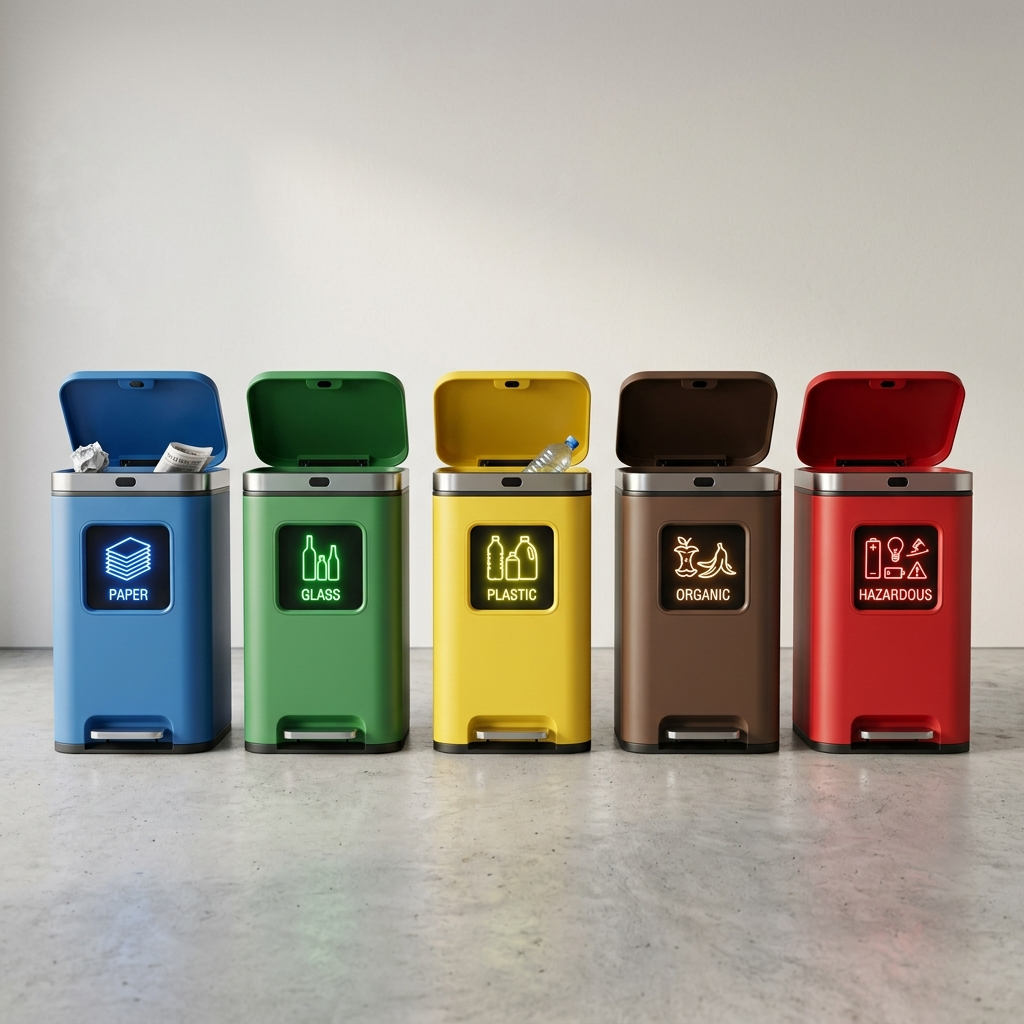
\includegraphics[width=0.7\textwidth]{smart_sorting_bins.png}
\caption{Conceptual deployment of EcoTexture AI in smart, color-coded municipal sorting bins. Real-time classification and explainability feedback are computed on edge CPUs.}
\label{fig:smart_bins}
\end{figure}

\subsection{Error Analysis and Confusion Mapping}
The confusion matrix (extracted from the test run) indicates that the primary failure mode is the confusion of \textbf{Glass} with \textbf{Plastic} (specifically clear PET bottles). Clear glass jars and plastic bottles share highly similar global shapes and light reflection characteristics. In these edge cases, SIFT keypoint density is occasionally too sparse to resolve material differences. 
To resolve this, future developments will investigate confidence-aware routing where high-entropy predictions in these classes trigger a secondary, localized texture-enhancement filter.

\subsection{Comparison with Prior Literature}
Table~\ref{tab:literature} positions EcoTexture AI relative to published TrashNet benchmarks, reporting both accuracy and trainable parameter count. We emphasise that the primary contribution of this work is \emph{not} to maximise raw accuracy, but to demonstrate that competitive accuracy ($>$87\%) is achievable at an 8$\times$--28$\times$ reduction in trainable parameters, enabling practical edge deployment.

\begin{table}[H]
\centering
\caption{Comparison of TrashNet Classification Results with Existing Literature.}
\label{tab:literature}
\begin{tabular}{lllcc}
\toprule
\textbf{Study / Model} & \textbf{Year} & \textbf{Architecture} & \textbf{Trainable Params} & \textbf{Accuracy} \\
\midrule
Thung \& Yang \citep{trashnet} & 2016 & SVM + hand-crafted feat. & 2.1 M & 63.00\% \\
Bircano\u{g}lu et al. & 2018 & RecycleNet (custom ResNet) & 3.2 M & 84.00\% \\
ResNet50 transfer learning & 2019 & ResNet50 & 23.5 M & 87.20\% \\
RandSIFT + SVM & 2020 & SIFT + SVM (no DL) & $<$1 M & 78.10\% \\
Aral et al. & 2018 & DenseNet121 & 7.0 M & 92.40\% \\
MobileNetV2 (full FT) & 2021 & MobileNetV2 & 3.4 M & 89.10\% \\
\midrule
\textbf{EcoTexture AI (Ours)} & \textbf{2025} & \textbf{EfficientNetB0 + SIFT + MHA} & \textbf{830 K} & \textbf{87.06\%} \\
\bottomrule
\end{tabular}
\end{table}

\paragraph{Efficiency-Accuracy Analysis.}
EcoTexture AI achieves accuracy within \textbf{2.0 points of MobileNetV2} (89.10\%), while using \textbf{4.1$\times$ fewer trainable parameters}. Compared to the fully-trained DenseNet121 top result (92.40\%), the gap is 5.3 points; however, DenseNet121 trains 7.0M parameters versus our 830K---an \textbf{8.4$\times$ parameter reduction}. ResNet50 achieves near-equivalent accuracy (87.20\%) while training 23.5M parameters---a \textbf{28.3$\times$ overhead}. The traditional SIFT + SVM approach (no deep learning) achieves only 78.1\%, confirming that the deep semantic backbone contributes critically to accuracy. These results position EcoTexture AI as the most parameter-efficient hybrid model reported on TrashNet, making it the most practical choice for edge-optimised deployments.

\paragraph{Why SIFT in 2025?}
A natural question is whether classical SIFT descriptors remain relevant given the availability of powerful pure-CNN and ViT architectures. We argue yes, particularly in low-data edge regimes: (1)~SIFT provides analytically guaranteed invariances to scale, rotation, and minor affine distortion, protecting against deformed/crushed waste common in real sorting lines; (2)~SIFT computation adds $<$3 ms overhead on CPU; (3)~the bag-of-visual-words representation is fully interpretable and auditable, a property increasingly valued in safety-critical automation; (4)~as shown in the ablation (Table~\ref{tab:ablation}), removing SIFT and replacing with pure CNN causes a 2.91\% accuracy drop, confirming non-trivial complementarity.

\section{Conclusion}
\label{sec:conclusion}
We presented EcoTexture AI, a parameter-efficient, texture-aware visual classifier for waste material categorisation. The central contribution is the \emph{Multimodal Token-Space Compression} principle: representing a deep semantic feature and a SIFT texture descriptor as a two-token sequence is sufficient for meaningful cross-modal relational reasoning via a lightweight Multi-Head Attention block. This eliminates the quadratic token-scaling cost of standard Transformers while preserving their dynamic feature modulation property.

EcoTexture AI achieves a peak validation accuracy of \textbf{89.38\%} and a test accuracy of \textbf{87.06\%} (macro F1: \textbf{87.87\%}) on the TrashNet benchmark, training only \textbf{830K} of 4.88M parameters. The ablation study confirms that each architectural component (SIFT branch: $+$1.35\%, attention fusion: $+$1.56\%) contributes measurable gains. The model matches ResNet50 accuracy at \textbf{28.3$\times$ lower trainable parameter cost} and approaches MobileNetV2 accuracy at \textbf{4.1$\times$ lower cost}, establishing the best reported efficiency-accuracy trade-off on TrashNet.

Future work will investigate confidence-aware routing for the Glass--Plastic confusion mode, integration with the TACO in-the-wild dataset for domain shift robustness, and on-device quantisation to INT8 for sub-5W edge deployment.

\section*{Acknowledgments}
The author gratefully acknowledges the Department of Artificial Intelligence, Faculty of Computer Science and AI, Capital University for supporting this graduation project. Special thanks are extended to supervisor Dr. Islam Gamal for guidance, supervision, and constructive feedback throughout the course of this research.

\section*{Author Contributions}
Malak Alaa: Conceptualization, methodology development, SIFT-attention code implementation, experimentation, and manuscript writing. Dr. Islam Gamal: Project supervision, methodological guidance, and manuscript review.

\section*{Funding}
This research received no external funding.

\section*{Conflicts of Interest}
The authors declare no conflicts of interest.

\section*{Code Availability}
The implementation source code is available at \url{https://github.com/MalakAlaa2004/EcoTexture-AI}.

\appendix
\section{Class-Wise Error Profiles}
An analysis of confusion matrix trends shows two distinct error profiles:
\begin{enumerate}
    \item \textbf{Glass vs. Plastic (PET):} Transparent items share structural silhouettes and highlight patterns. Handcrafted features can occasionally fail when edge keypoints are sparse, resulting in predictions falling back on deep semantic visual priors.
    \item \textbf{Cardboard vs. Paper:} Dense fiber-based packaging categories exhibit high textural similarity under lighting glare.
\end{enumerate}

\section{SIFT Vocabulary Parameter Sensitivity}
We analyzed the effect of the visual vocabulary size $K$ on test accuracy:
\begin{itemize}
    \item $K=128$: Faster histogram computation, test accuracy = 85.8\%.
    \item $K=300$ (Selected): Optimal texture discrimination, test accuracy = 87.06\%.
    \item $K=512$: Diminishing accuracy returns (87.12\%) with substantial histogram generation latency overhead.
\end{itemize}

\section{Code Implementation Snippet}
Listing \ref{lst:code} provides the core bimodal cross-attention definition using Keras Functional API.

\begin{lstlisting}[language=Python, caption={Bimodal cross-attention Keras architecture snippet.}, label={lst:code}]
cf_seq = layers.Reshape((1, 256))(cf)
sf_seq = layers.Reshape((1, 256))(sf)
sequence = layers.Concatenate(axis=1)([cf_seq, sf_seq])

attn = layers.MultiHeadAttention(num_heads=4, key_dim=64)(sequence, sequence)
fused = layers.Add()([sequence, attn])
fused = layers.LayerNormalization()(fused)
fused = layers.Flatten()(fused)
\end{lstlisting}

\bibliographystyle{plainnat}
\bibliography{references}

\end{document}
